\documentclass[11pt]{article}
\usepackage[margin=1in]{geometry}
\usepackage{graphicx}
\usepackage{amsmath}
\usepackage{amssymb}
\usepackage{float}
\usepackage{subcaption}
\usepackage{booktabs}

\title{September 15, 2021 Meeting Document}

\begin{document}
\maketitle

\section{Overview}
  This week I tried a couple more models to estimate the service rate. I tried the all-time min iterative model we discussed as well as a county fixed effects model, I have updated our results table to include them.
  An overview of the results are below.

  \begin{table}[H]
    \centering
    % \small
    \caption{Summary of Results}
    \begin{tabular}{llrr}
\toprule
      Model &         Group &  Pleas per Day &  Days per Trial \\
\midrule
        Min &        County &           6.92 &            4.41 \\
        Min &       Judge &           9.66 &            6.28 \\
        Min & Judge-County &          14.97 &            4.25 \\
  All time Min &        County &           7.12 &            3.65 \\
  All time Min &       Judge &           16.53 &            4.52 \\
  All time Min & Judge-County &          15.05 &            4.09 \\
Utilization &        County &           7.56 &            3.25 \\
Utilization &       Judge &          13.99 &            3.12 \\
Utilization & Judge-County &          20.90 &            1.73 \\
% Fixed Effects & Judge & 9.52 & 3.86 \\
% Fixed Effects & County & 10.99 & 4.34 \\
% Fixed Effects & Judge-County & 10.1 & 3.71 \\
\bottomrule
\end{tabular}

  \end{table}

\section{Iterative Idleness Estimation Taking All Time Mins}
  \textbf{Step 0:} We estimate the model, $\text{Days}_j = \beta_t\text{Trial}_j + \beta_p\text{Plea}_j +\epsilon_j$. \\

  \noindent \textbf{Steps 1-n:} We then use the estimates of $\beta^{(1)}_t$ and $\beta^{(1)}_p$ to estimate the expected number
  of days it would take each judge to complete their work. Mathematically: $\text{Expected Days}^{(1)}_j = \beta^{(1)}_p \cdot \text{Plea}_j + \beta^{(1)}_t \cdot \text{Trial}_j$.
  We would then set $\text{Days}^{(n)}_j = \min(\text{Days}_j,\text{Expected Days}^{(n-11)}_j,...,\text{Expected Days}^{(1)}_j)$ We then estimate the model $\text{Days}^{(1)}_j = \beta_t\text{Trial}_j + \beta_p\text{Plea}_j +\epsilon_j$ and repeat until convergence.

  \subsection{Judge Model}

    \begin{table}[H]
      \centering
      % \small
      \caption{Judge Model}
      \begin{center}
\begin{tabular}{lclc}
\toprule
\textbf{Dep. Variable:}    &        y         & \textbf{  R-squared:         } &     1.000   \\
\textbf{Model:}            &       OLS        & \textbf{  Adj. R-squared:    } &     1.000   \\
\textbf{Method:}           &  Least Squares   & \textbf{  F-statistic:       } & 1.813e+30   \\
\textbf{Date:}             & Tue, 14 Sep 2021 & \textbf{  Prob (F-statistic):} &     0.00    \\
\textbf{Time:}             &     13:26:30     & \textbf{  Log-Likelihood:    } &    1438.6   \\
\textbf{No. Observations:} &          50      & \textbf{  AIC:               } &    -2871.   \\
\textbf{Df Residuals:}     &          47      & \textbf{  BIC:               } &    -2865.   \\
\textbf{Df Model:}         &           2      & \textbf{                     } &             \\
\bottomrule
\end{tabular}
\begin{tabular}{lcccccc}
                   & \textbf{coef} & \textbf{std err} & \textbf{t} & \textbf{P$> |$t$|$} & \textbf{[0.025} & \textbf{0.975]}  \\
\midrule
\textbf{Intercept} &   -1.243e-14  &     2.56e-14     &    -0.485  &         0.630        &     -6.4e-14    &     3.91e-14     \\
\textbf{Plea}      &       0.0605  &     6.94e-17     &  8.72e+14  &         0.000        &        0.060    &        0.060     \\
\textbf{Trial}     &       4.5182  &        3e-15     &  1.51e+15  &         0.000        &        4.518    &        4.518     \\
\bottomrule
\end{tabular}
\begin{tabular}{lclc}
\textbf{Omnibus:}       &  8.336 & \textbf{  Durbin-Watson:     } &    2.156  \\
\textbf{Prob(Omnibus):} &  0.015 & \textbf{  Jarque-Bera (JB):  } &    7.538  \\
\textbf{Skew:}          & -0.791 & \textbf{  Prob(JB):          } &   0.0231  \\
\textbf{Kurtosis:}      &  4.056 & \textbf{  Cond. No.          } &     790.  \\
\bottomrule
\end{tabular}
%\caption{OLS Regression Results}
\end{center}

Notes: \newline
 [1] Standard Errors assume that the covariance matrix of the errors is correctly specified.
    \end{table}

    \begin{figure}[H]
      \centering
      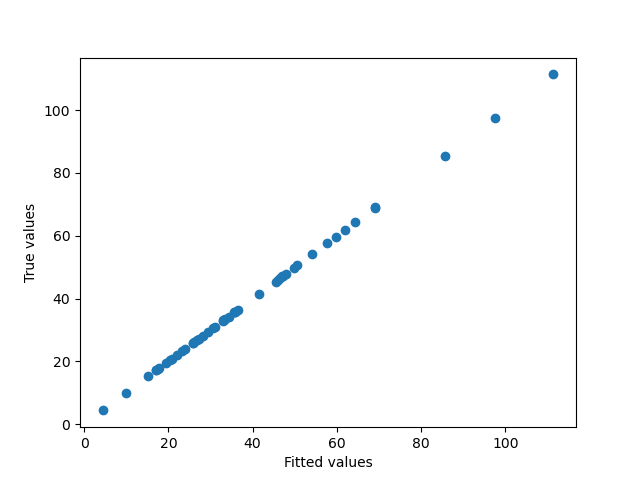
\includegraphics[width=0.65\textwidth]{../../../output/figures/Exploration/fit_min_JudgeID}
      \caption{True vs Fitted Values, Judge Model}
    \end{figure}

    \begin{table}[H]
      \centering
      % \small
      \caption{Judge Model}
      \begin{tabular}{rrr}
\toprule
 Iteration &  Beta P &  Beta T \\
\midrule
         0 &    0.06 &    4.52 \\
         1 &    0.06 &    4.52 \\
\bottomrule
\end{tabular}

    \end{table}

  \subsection{County Model}

    \begin{table}[H]
      \centering
      % \small
      \caption{County Model}
      \begin{center}
\begin{tabular}{lclc}
\toprule
\textbf{Dep. Variable:}    &        y         & \textbf{  R-squared:         } &     0.998   \\
\textbf{Model:}            &       OLS        & \textbf{  Adj. R-squared:    } &     0.998   \\
\textbf{Method:}           &  Least Squares   & \textbf{  F-statistic:       } & 1.342e+04   \\
\textbf{Date:}             & Tue, 14 Sep 2021 & \textbf{  Prob (F-statistic):} &  7.67e-61   \\
\textbf{Time:}             &     13:27:42     & \textbf{  Log-Likelihood:    } &   -115.16   \\
\textbf{No. Observations:} &          46      & \textbf{  AIC:               } &     236.3   \\
\textbf{Df Residuals:}     &          43      & \textbf{  BIC:               } &     241.8   \\
\textbf{Df Model:}         &           2      & \textbf{                     } &             \\
\bottomrule
\end{tabular}
\begin{tabular}{lcccccc}
                   & \textbf{coef} & \textbf{std err} & \textbf{t} & \textbf{P$> |$t$|$} & \textbf{[0.025} & \textbf{0.975]}  \\
\midrule
\textbf{Intercept} &       0.7176  &        0.599     &     1.199  &         0.237        &       -0.490    &        1.925     \\
\textbf{Plea}      &       0.1403  &        0.002     &    67.351  &         0.000        &        0.136    &        0.144     \\
\textbf{Trial}     &       3.6474  &        0.133     &    27.471  &         0.000        &        3.380    &        3.915     \\
\bottomrule
\end{tabular}
\begin{tabular}{lclc}
\textbf{Omnibus:}       & 68.690 & \textbf{  Durbin-Watson:     } &     2.097  \\
\textbf{Prob(Omnibus):} &  0.000 & \textbf{  Jarque-Bera (JB):  } &   840.457  \\
\textbf{Skew:}          & -3.638 & \textbf{  Prob(JB):          } & 3.14e-183  \\
\textbf{Kurtosis:}      & 22.636 & \textbf{  Cond. No.          } &      679.  \\
\bottomrule
\end{tabular}
%\caption{OLS Regression Results}
\end{center}

Notes: \newline
 [1] Standard Errors assume that the covariance matrix of the errors is correctly specified.
    \end{table}

    \begin{figure}[H]
      \centering
      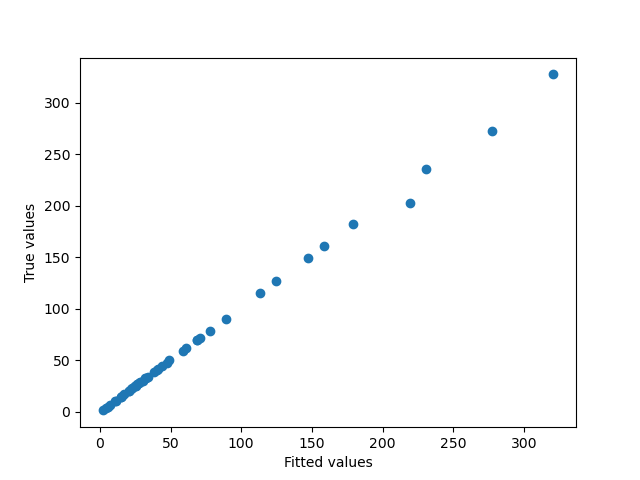
\includegraphics[width=0.65\textwidth]{../../../output/figures/Exploration/fit_min_County}
      \caption{True vs Fitted Values, Judge-County Model}
    \end{figure}

    \begin{table}[H]
      \centering
      % \small
      \caption{Judge Model}
      \begin{tabular}{rrr}
\toprule
 Iteration &  Beta P &  Beta T \\
\midrule
         0 &    0.15 &    3.61 \\
         1 &    0.14 &    3.67 \\
         2 &    0.14 &    3.65 \\
\bottomrule
\end{tabular}

    \end{table}

  \subsection{Judge-County Model}

    \begin{table}[H]
      \centering
      % \small
      \caption{County Model}
      \begin{center}
\begin{tabular}{lclc}
\toprule
\textbf{Dep. Variable:}    &        y         & \textbf{  R-squared:         } &     0.977   \\
\textbf{Model:}            &       OLS        & \textbf{  Adj. R-squared:    } &     0.977   \\
\textbf{Method:}           &  Least Squares   & \textbf{  F-statistic:       } &     5950.   \\
\textbf{Date:}             & Tue, 14 Sep 2021 & \textbf{  Prob (F-statistic):} & 4.56e-227   \\
\textbf{Time:}             &     13:28:16     & \textbf{  Log-Likelihood:    } &   -492.29   \\
\textbf{No. Observations:} &         278      & \textbf{  AIC:               } &     990.6   \\
\textbf{Df Residuals:}     &         275      & \textbf{  BIC:               } &     1001.   \\
\textbf{Df Model:}         &           2      & \textbf{                     } &             \\
\bottomrule
\end{tabular}
\begin{tabular}{lcccccc}
                   & \textbf{coef} & \textbf{std err} & \textbf{t} & \textbf{P$> |$t$|$} & \textbf{[0.025} & \textbf{0.975]}  \\
\midrule
\textbf{Intercept} &       0.4634  &        0.110     &     4.203  &         0.000        &        0.246    &        0.681     \\
\textbf{Plea}      &       0.0665  &        0.001     &    50.392  &         0.000        &        0.064    &        0.069     \\
\textbf{Trial}     &       4.0877  &        0.059     &    68.783  &         0.000        &        3.971    &        4.205     \\
\bottomrule
\end{tabular}
\begin{tabular}{lclc}
\textbf{Omnibus:}       & 462.896 & \textbf{  Durbin-Watson:     } &     2.072   \\
\textbf{Prob(Omnibus):} &   0.000 & \textbf{  Jarque-Bera (JB):  } & 159919.551  \\
\textbf{Skew:}          &  -8.673 & \textbf{  Prob(JB):          } &      0.00   \\
\textbf{Kurtosis:}      & 119.212 & \textbf{  Cond. No.          } &      116.   \\
\bottomrule
\end{tabular}
%\caption{OLS Regression Results}
\end{center}

Notes: \newline
 [1] Standard Errors assume that the covariance matrix of the errors is correctly specified.
    \end{table}

    \begin{figure}[H]
      \centering
      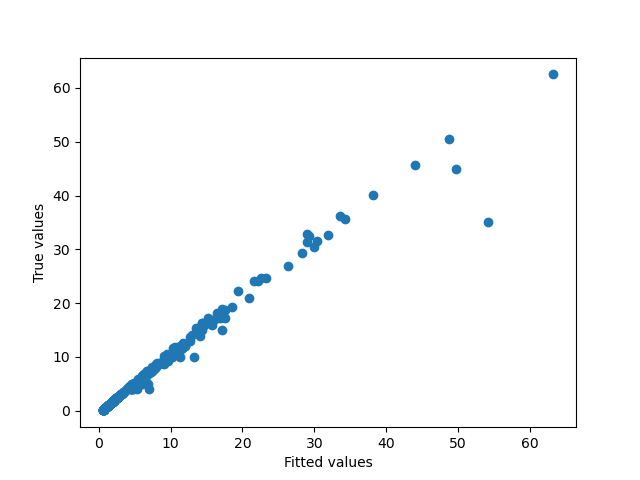
\includegraphics[width=0.65\textwidth]{../../../output/figures/Exploration/fit_min_JudgeIDCounty}
      \caption{True vs Fitted Values, Judge-County Model}
    \end{figure}

    \begin{table}[H]
      \centering
      % \small
      \caption{Judge-County Model}
      \begin{tabular}{rrr}
\toprule
 Iteration &  Beta P &  Beta T \\
\midrule
         0 &    0.10 &    4.19 \\
         1 &    0.08 &    4.11 \\
         2 &    0.07 &    4.09 \\
\bottomrule
\end{tabular}

    \end{table}

\section{Judge-level Busyness Analysis}
  The goal of this exercise was to get a better idea of which are the busiest judges.
  I focused only on GS days. So when I say the number of pleas and number of trials, I mean those that
  happened on GS days.
  We have at least three measures of business: the number of pleas, the number of trials, and
  the number of GS days assigned to a county. I ranked the judges according to a measure
  that combined the three measures. To create this measure, I ranked all of the judges according
  to each measure. I then multiplied each county's score in each measure to create an overall measure.
  So, for example, if Judge 1 had the most pleas, then its ranking according to pleas would be 1. If Judge 1 had the second most trials, then its ranking according to trials would be 2. If it had the sixth most GS days, then its ranking according to GS days would be 6. Judge 1's overall measure would be $1 \cdot 2 \cdot 6 = 12$. This ranking can be seen in table \ref{cdf-table}. I also created bar charts of the number of pleas, trials, GS days, and the utilization for each county. I calculate the utilization by using the service rate estimates from the county model to calculate the expected number of days it took to process each county's pleas and trials. I then divide the expected number of days by the actual number of assigned days to get the utilization.

  In table \ref{cdf-table}, the columns PleaShare, TrialShare, and GSShare
  contain the cumulative share of all pleas, trials, and GS days accounted for by the counties up to that row. So, for example, in the 10th row, if the value of PleaShare is 0.5, that means that the top
  10 counties account for $50\%$ of all pleas. Similarly, if in the 15th row the value of Trial share is 0.9, that means that the top 15 counties account for $90\%$ of all trials. GS share refers to the share of all GS days assigned. The counties in table \ref{cdf-table} are ranked using the measure described in the beginning of the section.

  \begin{table}[H]
    \centering
    \small
    \caption{CDF table}
    \label{cdf-table}
    \begin{tabular}{llrrrrrrr}
\toprule
{} &   JudgeID &  Plea &  Trial &   Days &  OverallScore &  PleaShare &  TrialShare &  GSDayShare \\
\midrule
1  &   Judge 7 &   572 &     17 & 167.00 &             4 &       0.04 &        0.08 &        0.04 \\
2  &  Judge 24 &   341 &     17 & 110.50 &           133 &       0.06 &        0.15 &        0.07 \\
3  &  Judge 50 &   469 &      9 & 129.50 &           144 &       0.09 &        0.19 &        0.10 \\
4  &  Judge 16 &  1041 &      5 &  90.00 &           320 &       0.16 &        0.21 &        0.12 \\
5  &  Judge 49 &   321 &      6 & 137.00 &           440 &       0.18 &        0.24 &        0.15 \\
6  &  Judge 18 &   202 &     11 & 123.00 &           576 &       0.19 &        0.29 &        0.18 \\
7  &   Judge 2 &   390 &      9 & 121.00 &           672 &       0.22 &        0.33 &        0.21 \\
8  &  Judge 11 &   244 &     12 & 107.00 &           810 &       0.23 &        0.38 &        0.24 \\
9  &   Judge 6 &   505 &      6 &  89.00 &          1056 &       0.27 &        0.41 &        0.26 \\
10 &  Judge 10 &   315 &      9 & 108.50 &          1232 &       0.29 &        0.45 &        0.28 \\
11 &  Judge 22 &   480 &      4 &  98.50 &          1848 &       0.32 &        0.47 &        0.31 \\
12 &  Judge 26 &   450 &      5 & 103.00 &          2052 &       0.35 &        0.49 &        0.33 \\
13 &   Judge 1 &   293 &      4 & 122.00 &          2300 &       0.37 &        0.51 &        0.36 \\
14 &  Judge 33 &   479 &      4 &  98.00 &          2352 &       0.40 &        0.52 &        0.39 \\
15 &  Judge 25 &   527 &      1 &  87.00 &          2898 &       0.43 &        0.53 &        0.41 \\
16 &   Judge 5 &   492 &      4 &  76.00 &          3360 &       0.47 &        0.55 &        0.42 \\
17 &  Judge 13 &   228 &      7 & 105.50 &          3410 &       0.48 &        0.58 &        0.45 \\
18 &  Judge 47 &   388 &      5 & 100.00 &          3536 &       0.51 &        0.60 &        0.47 \\
19 &  Judge 30 &   147 &     10 &  96.50 &          3870 &       0.52 &        0.64 &        0.50 \\
20 &   Judge 9 &   398 &      2 & 105.50 &          4800 &       0.54 &        0.65 &        0.52 \\
21 &  Judge 39 &   389 &      6 &  76.00 &          5655 &       0.57 &        0.68 &        0.54 \\
22 &  Judge 19 &   404 &      2 &  92.00 &          7524 &       0.59 &        0.69 &        0.56 \\
23 &  Judge 29 &   293 &      4 &  98.50 &          8280 &       0.61 &        0.71 &        0.59 \\
24 &   Judge 4 &   162 &      7 &  85.50 &          8856 &       0.62 &        0.74 &        0.61 \\
25 &  Judge 44 &   395 &      2 &  78.00 &         11934 &       0.65 &        0.75 &        0.63 \\
26 &  Judge 28 &   353 &      1 &  97.00 &         13464 &       0.67 &        0.75 &        0.65 \\
27 &   Judge 3 &   193 &      5 &  72.00 &         18870 &       0.68 &        0.77 &        0.67 \\
28 &   Judge 8 &   215 &      5 &  72.00 &         19008 &       0.70 &        0.80 &        0.68 \\
29 &  Judge 48 &   317 &      2 &  80.00 &         20202 &       0.72 &        0.80 &        0.70 \\
30 &  Judge 46 &   443 &      0 &  48.67 &         22050 &       0.75 &        0.80 &        0.71 \\
31 &  Judge 34 &   355 &      1 &  75.00 &         22950 &       0.77 &        0.81 &        0.73 \\
32 &  Judge 45 &   161 &      3 &  90.00 &         23814 &       0.78 &        0.82 &        0.75 \\
33 &  Judge 17 &   288 &      3 &  73.00 &         24025 &       0.80 &        0.84 &        0.77 \\
34 &  Judge 38 &   247 &      4 &  64.00 &         27550 &       0.82 &        0.85 &        0.79 \\
35 &  Judge 42 &   283 &      3 &  44.00 &         31772 &       0.84 &        0.87 &        0.80 \\
36 &  Judge 40 &   112 &      5 &  40.00 &         32256 &       0.84 &        0.89 &        0.81 \\
37 &  Judge 12 &   268 &      1 &  82.00 &         32900 &       0.86 &        0.89 &        0.83 \\
38 &  Judge 32 &   226 &      3 &  64.00 &         34336 &       0.88 &        0.91 &        0.84 \\
39 &  Judge 43 &   283 &      0 &  72.00 &         42768 &       0.89 &        0.91 &        0.86 \\
40 &  Judge 27 &   204 &      3 &  60.00 &         44800 &       0.91 &        0.92 &        0.87 \\
41 &  Judge 21 &   170 &      3 &  70.00 &         46200 &       0.92 &        0.93 &        0.89 \\
42 &  Judge 23 &   139 &      3 &  64.00 &         53820 &       0.93 &        0.95 &        0.91 \\
43 &  Judge 14 &   208 &      1 &  68.00 &         56304 &       0.94 &        0.95 &        0.92 \\
44 &  Judge 37 &   112 &      3 &  46.50 &         60536 &       0.95 &        0.96 &        0.93 \\
45 &  Judge 31 &   171 &      2 &  58.00 &         62361 &       0.96 &        0.97 &        0.95 \\
46 &  Judge 35 &   176 &      1 &  54.00 &         65436 &       0.97 &        0.98 &        0.96 \\
47 &  Judge 15 &   144 &      2 &  52.00 &         66220 &       0.98 &        0.99 &        0.97 \\
48 &  Judge 36 &   139 &      2 &  49.00 &         75240 &       0.99 &        1.00 &        0.99 \\
49 &  Judge 41 &    91 &      1 &  38.00 &        103243 &       1.00 &        1.00 &        0.99 \\
50 &  Judge 20 &    72 &      0 &  23.00 &        125000 &       1.00 &        1.00 &        1.00 \\
\bottomrule
\end{tabular}

  \end{table}


  \subsection{Overall Figures}
   In figure \ref{fig-county}, the counties are ordered according to the overall ranking described in the previous section.

    \begin{figure}[H]
      \centering
        \begin{subfigure}[b]{0.45\textwidth}
          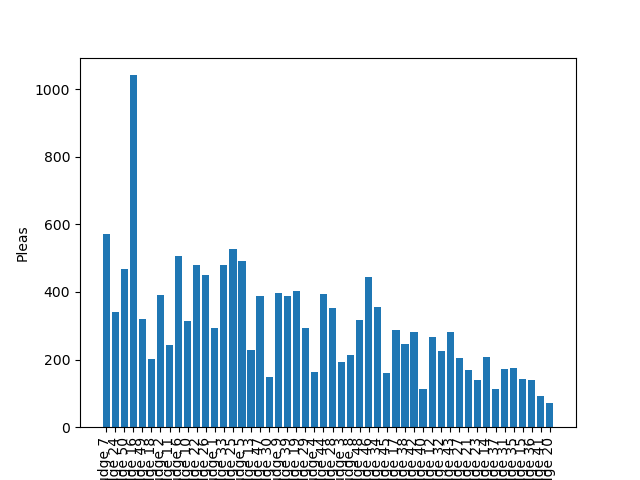
\includegraphics[width=\textwidth]{../../../output/figures/Exploration/judge_pleas.png}
          \caption{Pleas}
        \end{subfigure}
        \hfill
        \begin{subfigure}[b]{0.45\textwidth}
          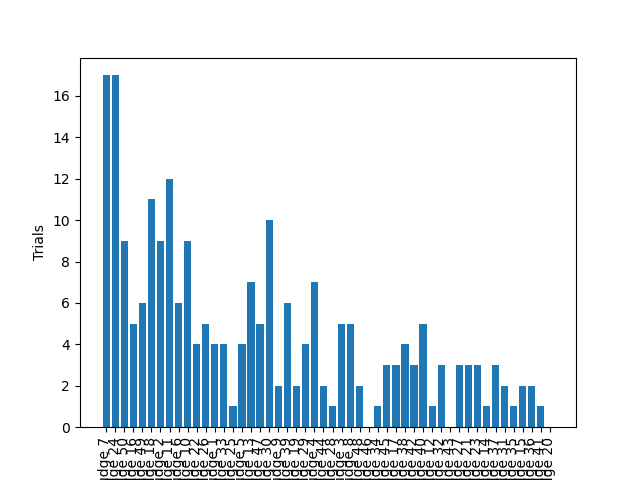
\includegraphics[width=\textwidth]{../../../output/figures/Exploration/judge_trials.png}
          \caption{Trials}

        \end{subfigure}
        %\hfill
        \begin{subfigure}[b]{0.45\textwidth}

          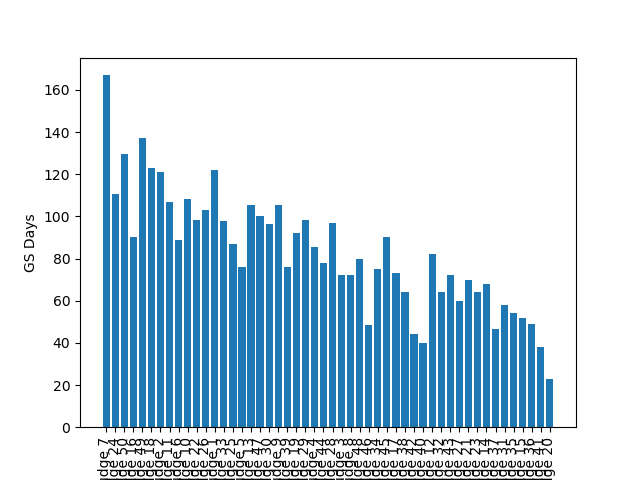
\includegraphics[width=\textwidth]{../../../output/figures/Exploration/judge_days.png}
          \caption{GS Days}

        \end{subfigure}
        \hfill
        \begin{subfigure}[b]{0.45\textwidth}

          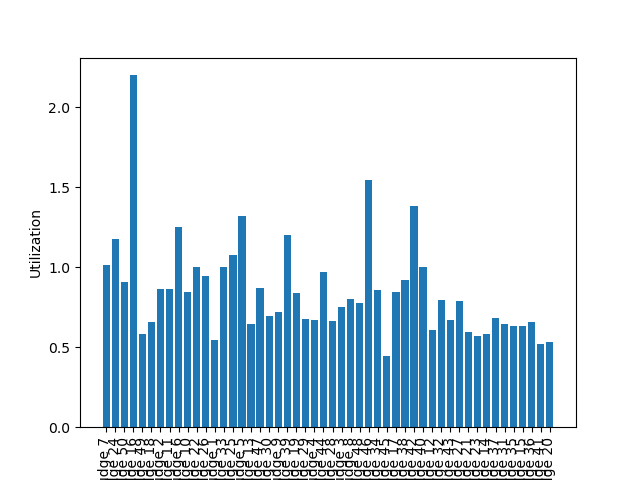
\includegraphics[width=\textwidth]{../../../output/figures/Exploration/judge_utilization.png}
          \caption{Utilization}

        \end{subfigure}
        \caption{Number of Pleas, Trials, GS days, and utilization for each county.}
        \label{fig-county}
    \end{figure}

  \subsection{Comparing Busy and Idle Judges}
    The purpose of this section is to further investigate how 'busy' counties are different from 'idle'
    counties. To do this, I split the counties into above median and below median in terms of business.
    Here, business is measured according to the measure described in the beginning of the section.

    \begin{figure}[H]
      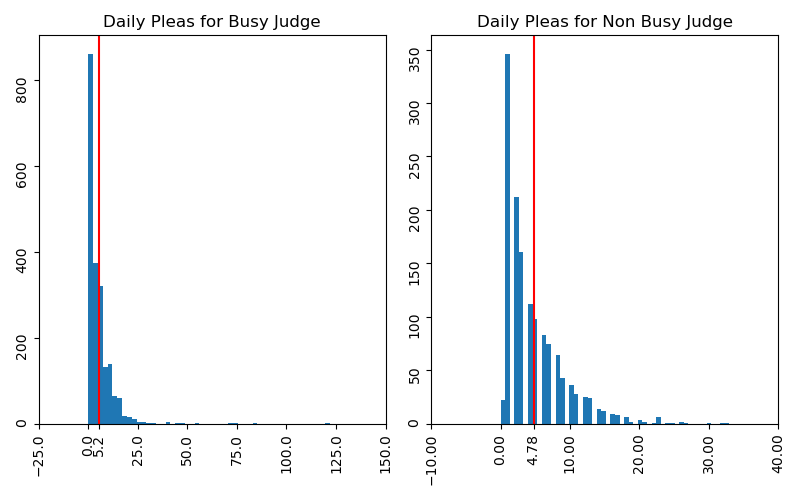
\includegraphics[width=0.9\textwidth]{../../../output/figures/Exploration/busy_vs_idle_judge_plea_hists.png}
      \caption{Histogram of pleas processed per day}
      \label{plea-hist}
    \end{figure}

\section{Model with County Fixed Effects}
  Note, the unit of observation here, $i$, is the judge-county combination. The regression we are running here is:  $\text{Days}_i = \alpha_c + \beta_p \text{Plea}_i + \beta_t \text{Trial}_i + \epsilon_i$

  \begin{figure}[H]
    \centering
    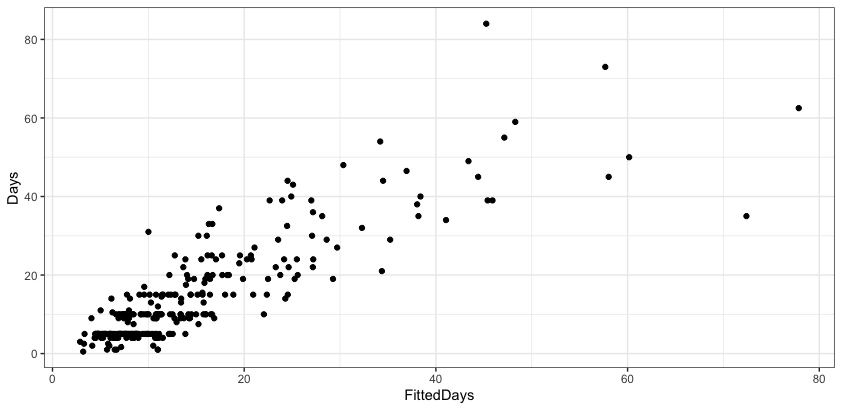
\includegraphics[width=0.65\textwidth]{../../../output/figures/Exploration/fit_fixed_County}
    \caption{True vs Fitted Values, fixed effects model}
  \end{figure}

  \begin{table}[H] \centering
    \caption{Model with County Fixed effects, table continues on next page}
    \small
    \begin{tabular}{@{\extracolsep{5pt}}lc}
    \\[-1.8ex]\hline
    \hline \\[-1.8ex]
     & \multicolumn{1}{c}{\textit{Dependent variable:}} \\
    \cline{2-2}
    \\[-1.8ex] & Days \\
    \hline \\[-1.8ex]
    Plea & 0.091$^{***}$ \\
     & (0.008) \\
     Trial & 4.336$^{***}$ \\
     & (0.339) \\
     CountyAbbeville & 6.411$^{*}$ \\
     & (3.784) \\
     CountyAiken & 3.107 \\
     & (2.909) \\
     CountyAllendale & 4.425 \\
     & (4.360) \\
     CountyAnderson & 5.237$^{*}$ \\
     & (2.985) \\
     CountyBamberg & 5.443 \\
     & (4.364) \\
     CountyBarnwell & 2.608 \\
     & (3.782) \\
     CountyBeaufort & 8.232$^{***}$ \\
     & (2.524) \\
     CountyBerkeley & 3.724 \\
     & (2.885) \\
     CountyCalhoun & 3.852 \\
     & (4.361) \\
     CountyCharleston & 9.165$^{***}$ \\
     & (2.237) \\
     CountyCherokee & 3.112 \\
     & (3.408) \\
     CountyChester & 14.170$^{***}$ \\
     & (4.365) \\
     CountyChesterfield & 4.966 \\
     & (3.093) \\
     CountyClarendon & 7.305$^{**}$ \\
     & (3.387) \\
     CountyColleton & 4.991$^{*}$ \\
     & (2.858) \\
     CountyDarlington & 7.293$^{**}$ \\
     & (3.091) \\
     CountyDillon & 7.260$^{**}$ \\
     & (3.380) \\
     CountyDorchester & 2.073 \\
     & (3.876) \\
     CountyEdgefield & 7.832$^{*}$ \\
     & (4.371) \\
     CountyFairfield & 5.677 \\
     & (3.798) \\
     CountyFlorence & 9.426$^{***}$ \\
     & (3.229) \\
     CountyGeorgetown & 5.565 \\
     & (3.415) \\
     CountyGreenville & 6.571$^{**}$ \\
     & (2.687) \\
     CountyGreenwood & 5.803$^{*}$ \\
     & (3.122) \\
     CountyHampton & 4.003 \\
     & (3.777) \\

     \hline \\[-1.8ex]
     Observations & 278 \\
     R$^{2}$ & 0.881 \\
     Adjusted R$^{2}$ & 0.856 \\
     Residual Std. Error & 7.552 (df = 230) \\
     F Statistic & 35.355$^{***}$ (df = 48; 230) \\
    \hline
    \hline \\[-1.8ex]
    \textit{Note:}  & \multicolumn{1}{r}{$^{*}$p$<$0.1; $^{**}$p$<$0.05; $^{***}$p$<$0.01} \\
    \end{tabular}
  \end{table}

  \begin{table}[H] \centering
    \caption{Model with County Fixed effects, continued}
    \small
    \begin{tabular}{@{\extracolsep{5pt}}lc}
    \\[-1.8ex]\hline
    \hline \\[-1.8ex]
     & \multicolumn{1}{c}{\textit{Dependent variable:}} \\
    \cline{2-2}
    \\[-1.8ex] & Days \\
    \hline \\[-1.8ex]
    CountyHorry & 5.715$^{**}$ \\
    & (2.482) \\
    CountyJasper & 3.514 \\
    & (3.779) \\
    CountyKershaw & 6.248$^{**}$ \\
    & (2.871) \\
    CountyLancaster & 11.090$^{***}$ \\
    & (3.788) \\
    CountyLaurens & 7.800$^{**}$ \\
    & (3.106) \\
    CountyLee & 4.218 \\
    & (3.382) \\
    CountyLexington & 4.390$^{**}$ \\
    & (2.219) \\
    CountyMarion & 5.295 \\
    & (3.790) \\
    CountyMarlboro & 10.937$^{***}$ \\
    & (3.792) \\
    CountyMcCormick & 6.248 \\
    & (4.362) \\
    CountyNewberry & 6.035$^{*}$ \\
    & (3.385) \\
    CountyOconee & 2.834 \\
    & (3.097) \\
    CountyOrangeburg & 6.506$^{**}$ \\
    & (2.689) \\
    CountyPickens & 6.166$^{**}$ \\
    & (3.101) \\
    CountyRichland & 10.717$^{***}$ \\
    & (2.141) \\
    CountySaluda & 4.655 \\
    & (4.365) \\
    CountySpartanburg & 2.984 \\
    & (2.897) \\
    CountySumter & 6.194$^{**}$ \\
    & (2.883) \\
    CountyUnion & 6.537$^{*}$ \\
    & (3.388) \\
    CountyWilliamsburg & 5.859$^{**}$ \\
    & (2.675) \\
    CountyYork & 7.085$^{***}$ \\
    & (2.651) \\
   \hline \\[-1.8ex]
  Observations & 278 \\
  R$^{2}$ & 0.881 \\
  Adjusted R$^{2}$ & 0.856 \\
  Residual Std. Error & 7.552 (df = 230) \\
  F Statistic & 35.355$^{***}$ (df = 48; 230) \\
    \hline
    \hline \\[-1.8ex]
    \textit{Note:}  & \multicolumn{1}{r}{$^{*}$p$<$0.1; $^{**}$p$<$0.05; $^{***}$p$<$0.01} \\
    \end{tabular}
  \end{table}

\section{Non-linear Approach}
  I looked into using a log-linear model, however, none of the approaches I found
  would yield simple to interpret service rates. I think we might be trading off
  more interpretable fixed effects for more interpretable service rate estimates.
  For example, we could estimate a Poisson regression with the specification
  $\text{Days}_i \sim P(\mu_i)$ and $\mu_i = \exp(\beta_p \text{Plea}_i + \beta_t\text{Trial}_i + \alpha_j)$.
  This would yield nice interpretations for the $\alpha_j$'s. The judge fixed effects would have a mutliplicative
  effect on the days, and we could interpret this as sort of proportional idleness. However, we would lose
  the simplicity of the model $\text{Days}_i = \beta_p \text{Trials}_i + \beta_p \text{Pleas}_i + \epsilon_i$. Since we are
  ultimately most interested in $\beta_p$ and $\beta_t$, I don't think this tradeoff is worth it.

\end{document}
